\section{Note compass}
Per quin motiu les escales són irregulars? Per què hi ha tecles blanques i negres en un piano i, a més a més, en un patró tan peculiar? Per què tenim una escala amb tons i semitons? Si hi donem una ullada més profunda, com s'agrupen les notes? Quin rol té cada grup? I més filosòficament, què transforma una seqüència de notes en música? Les respostes poden estar enterrades a la tradició i la notació musical, que poden semblar obscures i confuses. Aquest mòdul ens pot ajudar a orientar-nos i a trobar la lògica que s'hi amaga al darrere.

Sota la tradició musical occidental hi ha la idea que les notes disponibles, quan es miren de greu a agut, es repeteixen de forma cíclica.  Deixant de banda les consideracions acústiques, l'octava és el període de repetició de notes, anomenades d'aquesta manera perquè tradicionalment s'escullen 7 notes per cada cicle i la vuitena és, una altra vegada, la primera. Anomenem escala a aquesta selecció  de notes.

Una propietat fonamental de l'escala de la tradició occidental és que es genera amb un sol interval. Aquest interval generador és una distància entre notes que apareixen repetidament i, depenent de la seva mida, pot fer que les notes no quedin distribuïdes de forma equitativa. \footnote{No podem estar segurs de si l'escala es va inventar a partir aquesta propietat, ja que és lògicament equivalent a altres propietats musicals rellevants.}. Per fer la generació de l'escala comencem amb la primera nota i anem afegint l'interval generador per generar la segona nota, després només cal repetir el procés fins a obtenir 7 notes.  \footnote{Per experimentar amb altres intervals de generació i escales amb més o menys notes, dóna una ullada a la secció ``Scale Theory'' del mòdul Scale Lab.}. Aquest interval generador s'anomena quinta perfecta perquè, clàssicament, és la distància entre la primera i la cinquena nota de l'escala.

La propietat generadora en si és independent de l'acústica i no representa la mida actual de la quinta, però la tradició musical ha afavorit l'interval consonant. Al sistema tonal de dotze notes, que és una simplificació robusta i pràctica dels sistemes de notació tradicionals, l'aproximació és d'agafar un interval de quinta de 7/12 de la mida de l'octava.\footnote{Una octava s'associa acústicament a l'interval entre la freqüència f i el seu doble 2f. Normalitzant la mida de l'octava al logaritme log-freqüència 1 = log2(2), la quinta en afinació igual amb ràtio de freqüència 3:2 té mida log2(3/2)=0.58496. Això és molt proper al 7/12=0.58333. Hi ha una diferència d'aproximadament 0.16\%.}. Això significa que els intervals entre les nostres set notes són múltiples de la unitat bàsica de 1/12 de l'octava.

Gràficament, podem pensar en l'octava com un cercle i les unitats bàsiques de longitud 1/12 com els vèrtexs d'un dodecàgon. L'interval de quinta és un salt de 7 unitats bàsiques. Si unim tots els intervals de quinta (separats per 7/12 parts del cercle), obtenim una estrella de 12 puntes. D'aquesta manera, la nostra escala és una selecció de 7 dels 12 punts de l'estrella, units per una cadena de quintes.

També ens adonarem que alguns punts de l'escala són adjacents (a una distància d'una unitat) i altres deixen una distància de dues unitats (saltant alguns punts que no són a l'escala). Per les seves propietats aritmètiques, és impossible distribuir 7 de 12 punts uniformement sobre el dodecàgon, però les notes de la nostra escala estan distribuïdes de la manera més uniforme possible. Sempre trobem que hi ha 5 passos majors (dues unitats o el que anomenem un to) i dos passos menors (una unitat, anomenada semitò). Els passos menors se separen en grups de  dos i tres passos majors, respectivament. Aquesta escala és l'escala diatònica. Si tenim en compte l'inici i el final de l'escala ens trobem un dels següents patrons (anomenats modes) que reben noms grecs:

	2,2,1,2,2,2,1 - Jònic (major)
	2,1,2,2,2,1,2 - Dòric
	1,2,2,2,1,2,2 - Frigi
	2,2,2,1,2,2,1 - Lidi
	2,2,1,2,2,1,2 - Mixolidi
	2,1,2,2,1,2,2 - Eoli (minor)
	1,2,2,1,2,2,2 - Locri

Fixa't que tots els modes són permutacions cícliques dels altres, que significa agafar el primer element i posar-lo al final. Amb aquest model, per crear qualsevol mode concret només has de triar un dels 12 punts (la tònica) i un dels 7 patrons. Això et dóna  $12\cdot 7=84$ possibilitats. És important observar que el mode no és només el conjunt de set notes, també importa l'ordre i el seu punt de partida.

El mòdul Note Compass et permet visualitzar els 12 possibles modes diatònics. L'instrument consisteix en dos discs concèntrics. L'estrella de 12 puntes del davant representa les 12 notes de l'octava. La placa del darrere es divideix en sectors que et permeten seleccionar les notes. Les notes de l'estrella que estiguin al sector de color són part del mode, les que són al sector gris no hi són. El teclat de colors de l'aplicació només té les tecles per les notes de l'escala i no la resta.

Com es relacionen aquestes propietats aritmètiques i de combinatòria amb la música? Per una banda, per tocar aquestes notes els has d'assignar un to (o tipus de to) a cadascun dels 12 vèrtexs de l'estrella. El to exacte és un problema d'afinació o entonació que deixem de banda aquí, només remarquem que el to és un dels atributs de l'execució d'una nota.

Per  altra banda, les notes d'un mode es comporten com una família i interaccionen entre elles aconseguint un caràcter únic. La primera nota en un mode és la tònica, i serveix d'àncora per la resta de la família. Quan es diu que una peça està en Do Major significa que la seva tònica és el Do. Igualment, una peça en Do Menor té la mateixa tònica, però té un caràcter diferent. És a dir, tot i tenir la mateixa tònica, els diferents modes tenen caràcters molt diferents. Per tant, l'ordre de les notes dins del mode i la relació entre els salts majors i menors també són atributs d'una nota que es tenen en compte dins la lògica d'una composició. 


Amb aquests atributs, hi ha tres maneres de referir-se a una nota:

\begin{enumerate}

\item Els noms A, B, C, D, E, F, G (possiblement amb sostinguts o bemolls) indiquen el to que s'ha de tocar. Es fixa tan bon punt el teu instrument està afinat. Per exemple, en l'afinació de temperament igual, el A (o La) central té 440 Hz. Els noms de les notes apareixen a les dotze agulles del dodecàgon en forma d'estrella.

\item Els numerals aràbics 1, 2, 3, 4, 5, 6, 7, (8 = 1) designen la seva posició (graus d'escala) en una escala en ordre ascendent. El grau 1 es refereix a la nota que governa musicalment la col·lecció dels set graus.  Cada numeral es correspon a un dels segments de colors del disc exterior del Tone Compass (1 = Vermell, 2 = Taronja, 3 = Groc, 4 = Verd clar, 5 = Verd fosc, 6 = Blau fosc, 7 = Violeta). A qualsevol configuració del Note Compass hi ha exactament set de les 12 agulles apuntant a aquests segments de colors i, per tant, als set graus 1, 2, 3, 4, 5, 6 i 7. 

\item Les síl·labes do, re, mi, fa, so, la, si designen els caràcters de les set notes i tenen lloc a punts concrets respecte als dos passos menors al patró d'intervals. Els passos menors (d'un semitò) sempre es troben entre el mi i el fa i entre si i do. Podem pensar en cada mode com una petita societat de notes on s'atribueix un caràcter únic a cada nota. Al Note Compass, les set síl·labes apareixen entre les petites subdivisions de cada segment de colors en ordre antihorari fa - do - sol - re - la - mi - si. Qualsevol configuració del Note Compass farà que les set agulles actives (que apunten a segments de color) apuntin precisament a una de les set síl·labes. 

\end{enumerate}

Fixa't que els noms són:

C, C\#/Db, D, D\#/Eb, E, F, F\#/Gb, G, G\#/Ab, A, A\#/Bb, B.

La notació es basa essencialment en l'escala diatònica, i s'ancora en una família particular de modes on les notes s'anomenen amb les lletres A, B, C, D, E, F, G. Es corresponen a les tecles blanques del piano. Tota la resta de notes tenen alteracions \# (sostinguts) o b (bemolls) al seu nom. Per exemple, A\# és una nota més aguda que A, Bb és una nota més greu que B. El nombre d'alteracions és la diferència entre un pas major i un de menor i, en el sistema de dotze notes, A\# i Bb són idèntics i, per tant, es troben a la mateixa agulla de l'estrella del Note Compass.  

Les set notes d'un mode diatònic es representen generalment en set graus d'alçada successius en un pentagrama. Els noms de les notes sempre recorren els set noms A, B, C, D, E, F, G (Molt possiblement acompanyats de les l'alteració sostingut \# o bemoll b). La posició dels passos majors o menors no es representen gràficament en una partitura, els músics ja els saben veient la clau.

Això és un tribut a la tradició, al fet que tot els modes són elements i, alhora, alteracions d'una mateixa escala (que actualment anomenem Do Major).

Anem a veure un exemple del funcionament del Note Compass. Comencem amb l'escala més habitual: Do Major (o Do Jònic). Apunta l'agulla amb el Do cap al sector vermell que apunta cap a la síl·laba Do. Tenim aquesta ja coneguda concordança:

C -> (1, do), D -> (2, re), E -> (3, mi), F -> (4, fa) , G -> (5,so), A -> (6, la), B -> (7, si)

Fixa't que les agulles actives són (des del 1r sector fins al 7è), ordenades per passos, 2,2,1,2,2,2,1 (mode Jònic). El pas menor (d'un semitò) apareix quan dues agulles consecutives estan actives. 

Ara rota l'estrella una posició en direcció antihorària. L'agulla B que apunta cap a (7, si) deixa el segment violeta i apunta cap a un segment gris entre el violeta i el vermell. Ara ja no és una nota activa en aquest mode. En canvi, l'agulla Bb entra des d'una zona grisa cap a la violeta i apunta cap a la síl·laba Fa. El pas menor (si-do) entre B i C es transforma en un pas major (fa-sol) entre Bb i C i el pas major (la-si) entre A i B es transforma en un pas menor (mi-fa) entre A i Bb. El patró d'intervals és 2,2,1,2,2,1,2 (mode Mixolidi) 

És crucial que amb cada rotació elemental només una agulla es desselecciona i una de nova (adjacent a aquesta) es selecciona, per tant, només s'altera una nota de l'escala. Aquest fet té el seu origen en la irregularitat del patró que segueix l'escala diatònica. Matemàticament, és una permutació cíclica del patró que també es pot obtenir intercanviant passos adjacents (una transposició). A continuació hi ha una demostració d'aquesta peculiaritat: Si rotem el nom de l'exposició lalalab quatre lletres a l'esquerra obtenim  lablala. Si fem l'intercanvi de les últimes dues lletres, lalalba, que són clarament diferents de lablala. De totes maneres, si apliquem aquestes dues transformacions al patró Jònic 2212221, obtenim 2212212 en els dos casos. 

Aquesta propietat es reflecteix en com els músics utilitzen la clau i a la partitura per escriure-hi el mode, normalment afegint sostinguts o bé bemolls.

Finalment, cal fer alguns aclariments sobre nomenclatura de les diferents tradicions europees per evitar confusió: Per començar, als indrets germànics, les notes Si i Sib s'anomenen H i B, respectivament. Etimològicament, això prové del b quadratum i el b rotundum que s'han mantingut a la tradició. També, a la majoria d'idiomes Romànics i Eslaus, les síl·labes do, re, mi, fa sol, la si s'han utilitzat per substituir les lletres C, D, E, F, G, A, B al seu rol d'anomenar les notes. Això es remunta a l'any 1600 a França, tot i que les síl·labes ut, re, mi, fa i sol van aparèixer molt abans, al voltant de l'any 1000 amb Guido D'Arezzo.


Tot i les diferències en nomenclatura i ensenyament, les tradicions musicals són conscients de la importància de les tres especificacions de la nota (alçada del to, grau, i caràcter modal). El Tone Compass expressa la natura de la seva independència. Per l'amant de la música, pot ser instructiu entendre aquesta notació musical i practicar amb la tradició, percepció i aritmètica que encapsula. 


\begin{figure}[hp]
\centering
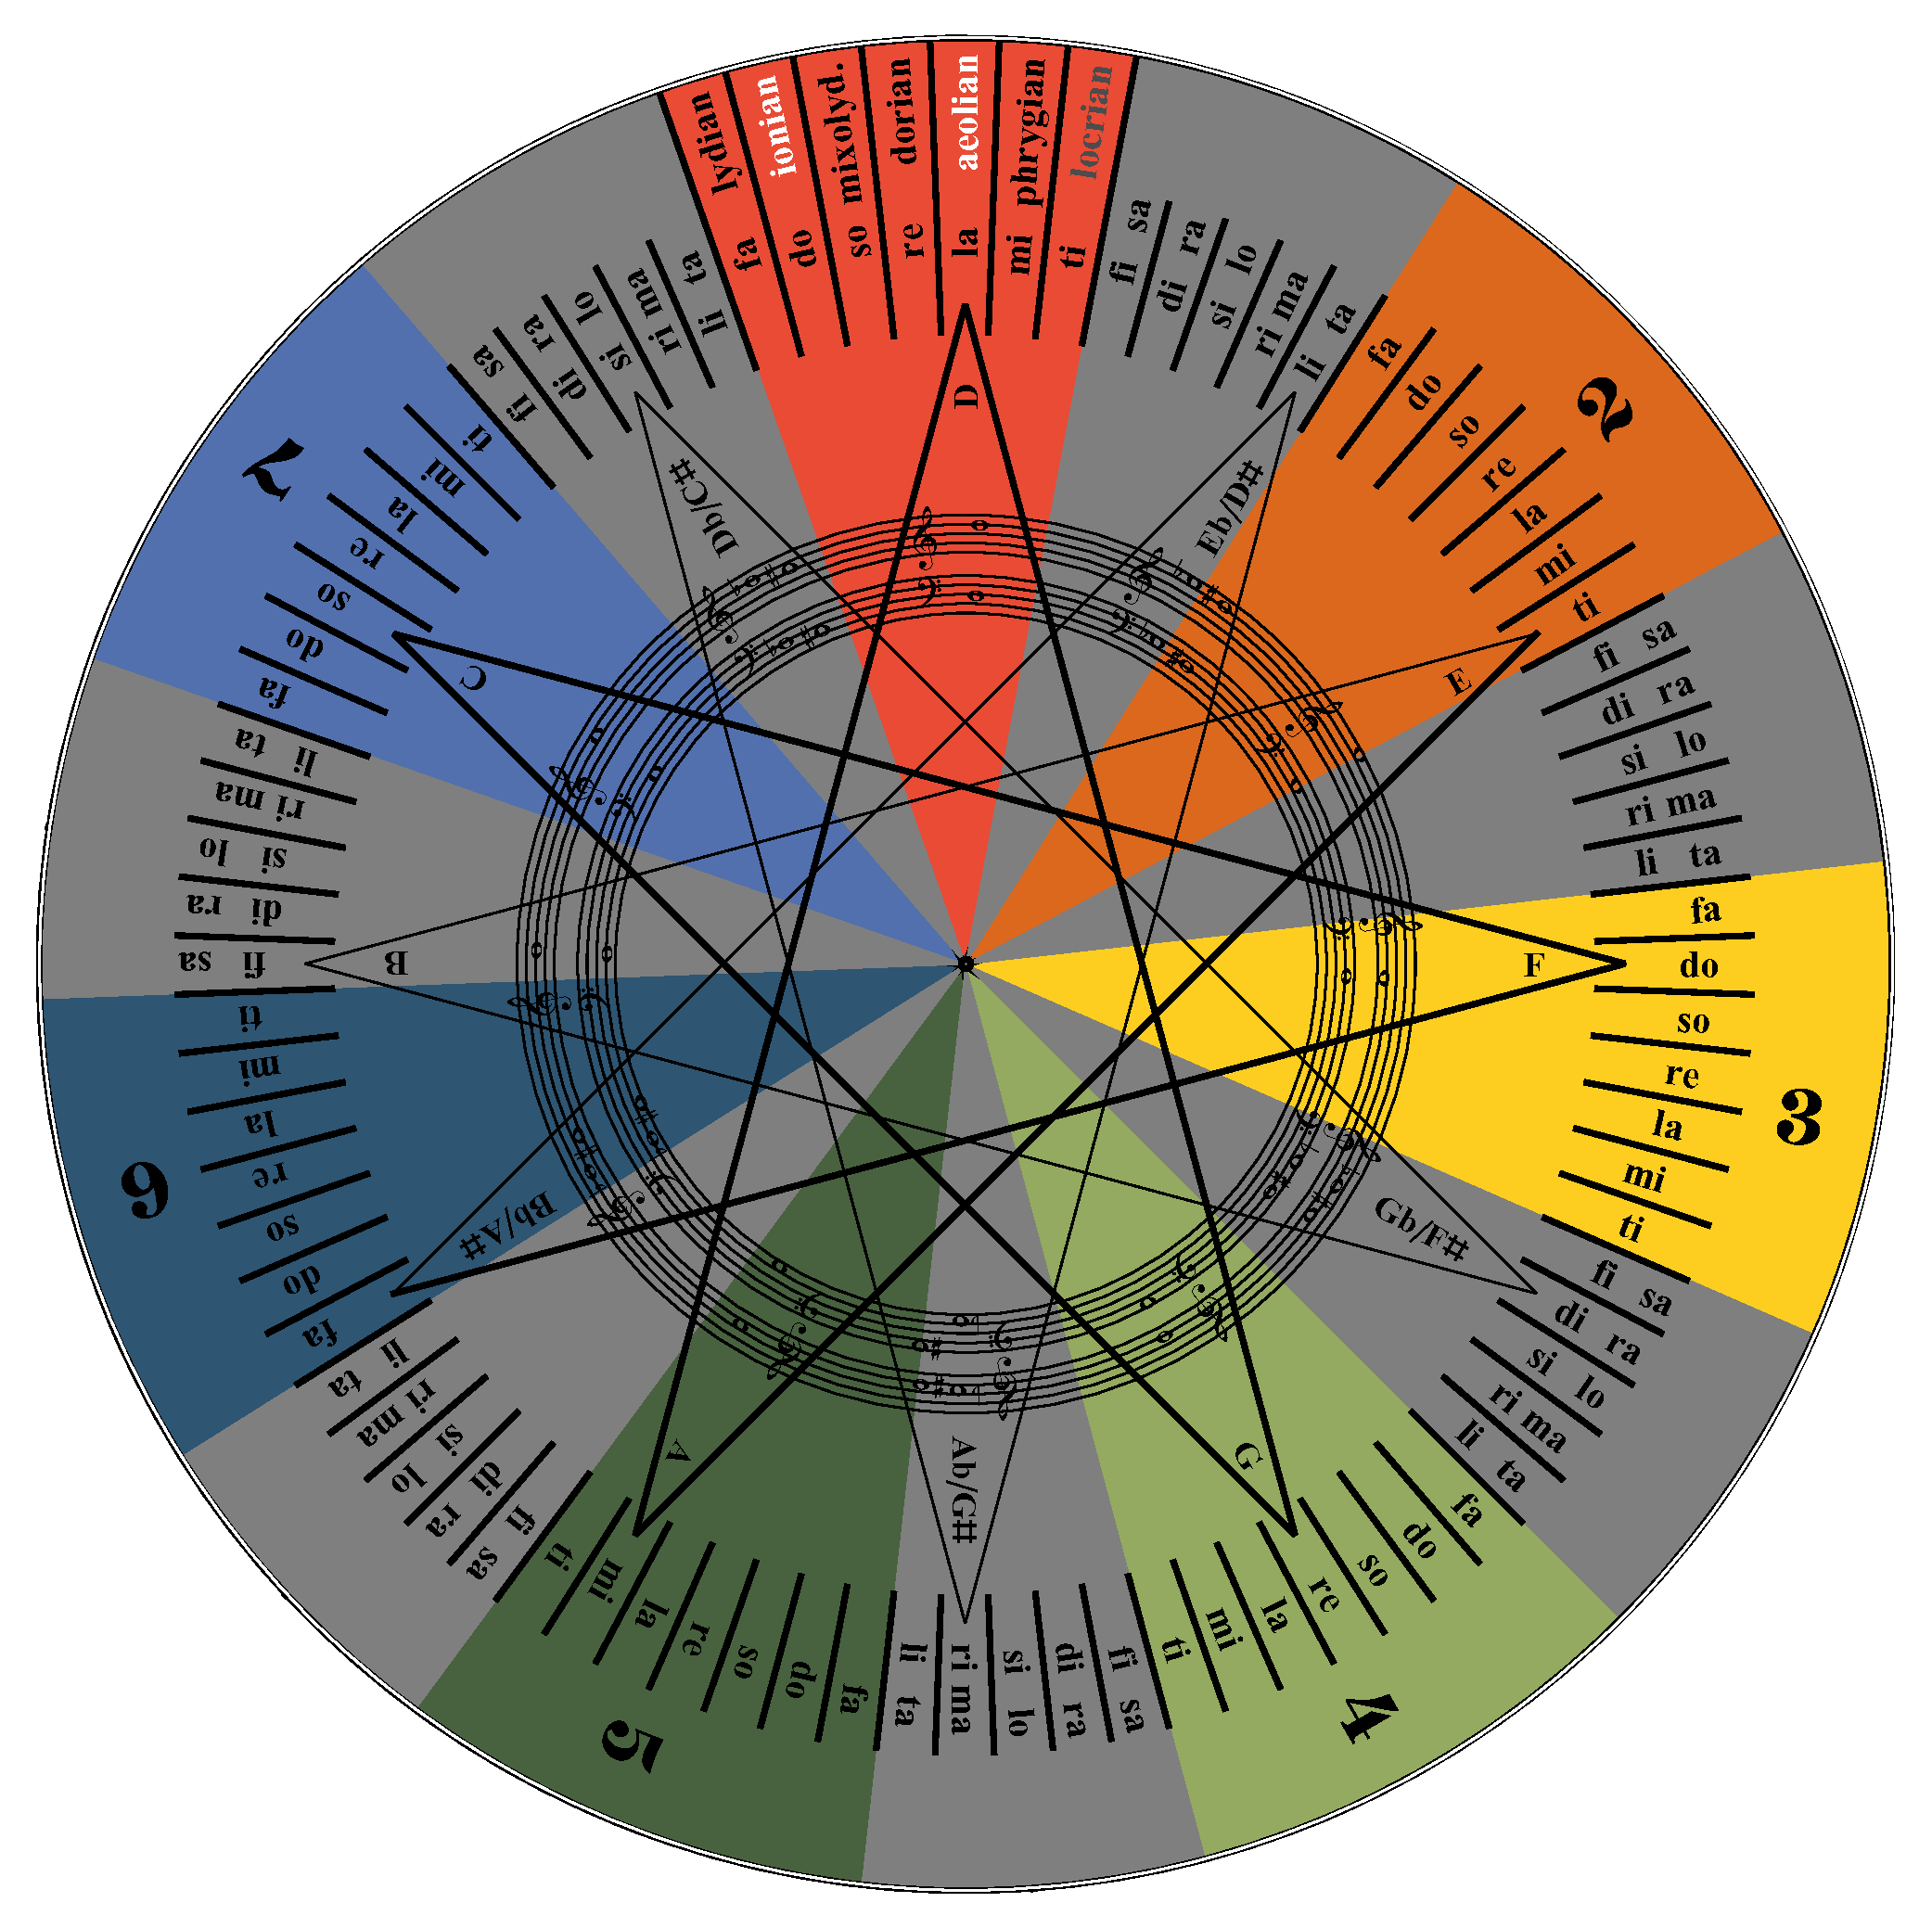
\includegraphics[width=0.95\textwidth]{NoteCompass_1}
\caption*{El Note Compass mostrant Re-Eoli. Les línies més gruixudes de l'estrella marquen la cadena de quintes de l'escala.}
\end{figure}


\vfill

Autors del mòdul: Thomas Noll (concepte) i Daniel Ramos per a IMAGINARY (Implementació).
Text: Thomas Noll i Daniel Ramos.
